\documentclass[12pt]{article}
\usepackage{graphicx}
\usepackage{xcolor}
\usepackage{hyperref}
\usepackage{wasysym}
\usepackage{mathrsfs}
\usepackage[calc]{datetime2}
\usepackage{boondox-cal}
\usepackage{bm} % For bold math symbols
\usepackage{amsmath,amsthm,amssymb,amsbsy}
\usepackage{gensymb}
\usepackage{cancel}
\usepackage{tikz}
\usetikzlibrary{3d,calc}
\usetikzlibrary{arrows}

\DTMsavenow{now}
\DTMsavedate{DueDate}{2024-02-21}

\newcount\daystilldue
\newcount\hourstilldue
\newcount\minutestilldue

% Calculate the difference in days
\DTMsaveddatediff{DueDate}{now}{\daystilldue}

% Calculate the difference in hours and minutes
\hourstilldue=\DTMfetchhour{DueDate}
\advance\hourstilldue by -\DTMfetchhour{now}
\minutestilldue=\DTMfetchminute{DueDate}
\advance\minutestilldue by -\DTMfetchminute{now}

% Adjust for negative values
\ifnum\hourstilldue<0
  \advance\hourstilldue by 24
  \advance\daystilldue by -1
\fi
\ifnum\minutestilldue<0
  \advance\minutestilldue by 60
  \advance\hourstilldue by -1
\fi

\newcommand{\TimeUntilDue}{
  \ifnum\daystilldue<4
    \textcolor{red}{
    \number\daystilldue\ days - 
    \number\hourstilldue\ hours - 
    \number\minutestilldue\ min until deadline!!
  }
\else
    \number\daystilldue\ days - 
    \number\hourstilldue\ hours - 
    \number\minutestilldue\ min until deadline
  \fi
}



% Save the original \BibTeX command in case you need it later
\let\originalBibTeX\BibTeX

% Redefine the \BibTeX command to display the LaTeX logo
\renewcommand{\BibTeX}{{\rmfamily B\kern-.03em{\sffamily ib}\kern-.15em\TeX}}


\newcommand{\delCross}[1]{
  \left[\hat a_x\left(\frac{\partial\bm{#1}_z}{\partial y} - \frac{\partial\bm{#1}_y}{\partial z}\right) - \hat a_y\left( \frac{\partial\bm{#1}_z}{\partial x} - \frac{\partial\bm{#1}_x}{\partial z}  \right) + \hat a_z\left( \frac{\partial\bm{#1}_y}{\partial x} -  \frac{\partial\bm{#1}_x}{\partial y}\right)\right]
}
\begin{document}

\newcommand{\Cross}[2]{
\hat a_x(#1_2#2_3 -#1_3#2_2) -\hat a_y(#1_1#2_3-#1_3#2_1) + \hat a_z(#1_1#2_2-#1_2#2_1) 
}
\title{ECE 6310 - Advanced Electromagnetic Fields: Homework Set \#3}
\author{Miguel Gomez}
%\date{\TimeUntilDue}
\maketitle

%\begin{center}
%  $\mathcal{ABCDEFGHIJKLMNOPQRSTUVWXYZ}$\\
%$\mathscr{ABCDEFGHIJKLMNOPQRSTUVWXYZ}$
%\end{center}
\section*{Preliminaries}
In this document, we use standard notation for electromagnetic theory. Key equations and concepts are summarized below:

\subsection*{Vector Notation}
\begin{itemize}
  \item $\bm{\mathcal{E}}$: Electric field intensity
  \item $\bm{\mathcal{H}}$: Magnetic field intensity
  \item $\bm{\mathcal{D}}$: Electric flux density
  \item $\bm{\mathcal{B}}$: Magnetic flux density
  \item $\bm{\mathcal{J}}$: Current density
  \item $\rho_v$: Volume charge density
\end{itemize}

\subsection*{Differential Operators}
\begin{itemize}
  \item $\nabla \cdot\ \ $: Divergence of a vector field
  \item $\nabla \times\ \ $: Curl of a vector field
  \item $\nabla\ \ $: Gradient of a scalar field
  \item $\partial_i\ \ $: Partial derivative with respect to the independent basis element $i$
\end{itemize}

\subsection*{Maxwell's Equations}
In integral form, Maxwell's equations are given by:
\begin{align}
  \oint_{\partial V} \bm{\mathcal{E}} \cdot d\bm{\mathcal{l}} &= - \frac{d}{dt} \int_{V} \bm{\mathcal{B}} \cdot d\bm{\mathcal{S}} & \text{(Faraday's Law of Induction)} \\
  \oint_{\partial V} \bm{\mathcal{H}} \cdot d\bm{\mathcal{l}} &= \int_{V} \bm{\mathcal{J}} \cdot d\bm{\mathcal{S}} + \frac{d}{dt} \int_{V} \bm{\mathcal{D}} \cdot d\bm{\mathcal{S}} & \text{(Ampère's Circuital Law)} \\
  \oiint_{\partial V} \bm{\mathcal{D}} \cdot d\bm{\mathcal{S}} &= \int_{V} \rho_v dV & \text{(Gauss's Law for Electricity)} \\
  \oiint_{\partial V} \bm{\mathcal{B}} \cdot d\bm{\mathcal{S}} &= 0 & \text{(Gauss's Law for Magnetism)}
\end{align}

\subsection*{Other Relevant Equations}
\begin{itemize}
  \item Continuity Equation: $\nabla \cdot \bm{\mathcal{J}} + \partial_t \rho_v = 0$
  \item Relationship between $\bm{\mathcal{E}}$, $\bm{\mathcal{D}}$: $\bm{\mathcal{D}} = \epsilon \bm{\mathcal{E}}$
  \item Relationship between $\bm{\mathcal{H}}$, $\bm{\mathcal{B}}$: $\bm{\mathcal{B}} = \mu \bm{\mathcal{H}}$
\end{itemize}

\subsection*{Boundary Conditions}
Discuss the boundary conditions for $\bm{\mathcal{E}}$, $\bm{\mathcal{H}}$, $\bm{\mathcal{D}}$, and $\bm{\mathcal{B}}$ at interfaces between different media.
\newpage
\section{- 6.19}
Show that for observations made at very large distances $(\beta r \gg 1)$ the electric and magnetic fields of Example 6-3 reduce to the following:
\begin{center}
  \begin{align*}
    E_{\theta} &= j\eta \frac{\beta \bm{I}_e\ell e^{-j\beta r}}{4 \pi r} \sin{(\theta)}\\
    H_{\phi} &\approx \frac{E_{\theta}}{\eta}\\
    E_{r} &\approx 0\\
    E_{\phi} &= H_r = H_{\theta} = 0
  \end{align*}
\end{center}
All of the above can be found bf considering a typical hertzian dipole. The example shows that we have an infinitesimal dipole with the length much smaller than a wavelength $\lambda$. Therefore, we can take the expressions as shown with all parts $E$ and $H$ getting a factor of $e^{-j\beta R}$ for the decay, and will have another dependent on the distance from the location of the dipole. We can ignore the factors present in all the values and look to only the factors containin $r^{-1}$.
\begin{align*}
  E_{r} &= A\cdot \left(\frac{1}{r^2}\right)\left(1 + \frac{1}{j\beta r}\right)\\
  &= \left(\frac{1}{r^2} + \frac{1}{j\beta r^3}\right)
\end{align*}
With $r$ being much greater than 1, we can approximate that $E_r \xrightarrow{} 0$ as the distance gets larger.
\begin{align*}
  H_r &= H_{\theta} = 0
\end{align*}
These follow from the reduction of the vector potential equation after converting to spherical. With $A_{phi} = 0$, we do not end up with components in the H direction for these. Then, $H_{phi}$ contains the same factors discussed above and we ignore the ones with higher order $r$'s in the denominator. Leaving us with the same constant multiplied across all terms, but divided by $\eta$, which substituting $E_{theta}$ for that factor gives the expected $H_{phi} \xrightarrow{} \frac{E_{theta}}{\eta}$
\newpage
\section{- 6.20}
For 6.19, show that
\begin{itemize}
\item the time average power density is:
  \begin{align*}
    \mathbf{S} &= \frac{1}{2}\text{Re}{[\mathbf{E}\times\mathbf{H}^*]} = \hat a_r W_{av} = \hat a_r W_{r}\\
    [\mathbf{E}\times\mathbf{H}^*] &= \frac{a_r}{r\sin{\left(\theta\right)}}\left(E_{\theta}H^*_{\phi}-E_{\phi}H^*_{\theta}\right) - \frac{a_\theta}{r}\left(E_{r}H^*_{\phi}-E_{\phi}H^*_{r}\right) + \frac{a_\phi}{r}\left(E_{r}H^*_{\theta}-E_{\theta}H^*_{r}\right)\\
    [\mathbf{E}\times\mathbf{H}^*] &= \frac{a_r}{r\sin{\left(\theta\right)}}\left(E_{\theta}\frac{E^*_{\theta}}{\eta}-E_{\phi}0\right) - \frac{a_\theta}{r}\left(0\frac{E^*_{\theta}}{\eta}-E_{\phi}0\right) + \frac{a_\phi}{r}\left(00-E_{\theta}0\right)\\
    \frac{1}{2}[\mathbf{E}\times\mathbf{H}^*] &= \frac{a_r}{2r\sin{\left(\theta\right)}}\left(E_{\theta}\frac{E^*_{\theta}}{\eta}\right) = \frac{a_r}{2r\eta\sin{\left(\theta\right)}}\left(E_{\theta}E^*_{\theta}\right)\\
    \frac{1}{2}[\mathbf{E}\times\mathbf{H}^*] &= \frac{a_r}{2r\sin{\left(\theta\right)}}\left(E_{\theta}\frac{E^*_{\theta}}{\eta}\right) \\
    &= \frac{a_r}{2r\eta\sin{\left(\theta\right)}}\left(\left|j\eta \frac{\beta \bm{I}_e\ell e^{-j\beta r}}{4 \pi r} \sin{(\theta)}\right|\right)^2\\
    &= \frac{a_r}{2r\eta\sin{\left(\theta\right)}}\left(\eta \frac{\beta \bm{I}_e\ell}{4 \pi r}\right)^2 \sin{(\theta)}^2\\
    &= a_r\frac{\eta}{2r\sin{\left(\theta\right)}}\left( \frac{ \bm{I}_e\ell}{2 \lambda r}\right)^2 \sin{(\theta)}^2\\
    &= a_r\frac{\eta}{8r^3\sin{\left(\theta\right)}}\left( \frac{ \bm{I}_e\ell}{\lambda}\right)^2 \sin{(\theta)}^2\\
    &= a_r\frac{1}{r\sin{\left(\theta\right)}}\frac{\eta}{8}\left| \frac{ \bm{I}_e\ell}{\lambda}\right|^2 \left(\frac{\sin{(\theta)}}{r}\right)^2
  \end{align*}
  It appears I included an erroneous factor of $\frac{1}{r\sin{\left(\theta\right)}}$. I believe that came from the conversion to spherical cross product. 
\item Radiation Intensity
    \begin{align*}
      \mathbf{U} &= r^2S_{av} = \frac{\eta}{8}\left|\frac{\mathbf{I}_o\ell}{\lambda}\right|^2  \sin{(\theta)}^2= r^2a_r\frac{\eta}{8}\left| \frac{ \bm{I}_e\ell}{\lambda}\right|^2 \left(\frac{\sin{(\theta)}}{r}\right)^2 \\
                 &= a_r\frac{\eta}{8}\left| \frac{ \bm{I}_e\ell}{\lambda}\right|^2 \sin{(\theta)}^2
    \end{align*}
\item Radiated Power
    \begin{align*}
      \mathbf{P}_{rad} &= \int_0^{2\pi}\int_0^{\pi}\mathbf(U)(\theta,\phi)\times \sin{(\theta)}d\theta d\phi = \eta\left(\frac{\pi}{3}\right)\left|\frac{\mathbf{I}_o\ell}{\lambda}\right|^2\\
      \mathbf{P}_{rad} &= \int_0^{2\pi}\int_0^{\pi}a_r\frac{\eta}{8}\left| \frac{ \bm{I}_e\ell}{\lambda}\right|^2 \sin{(\theta)}^3d\theta d\phi \\
      \sin^2{\theta} + \cos^2{\theta} &= 1 \xrightarrow{\ \ \ \ \ } \sin^2{\theta} = 1 - \cos^2{\theta}\\
      \mathbf{P}_{rad} &= \int_0^{2\pi}\int_0^{\pi}a_r\frac{\eta}{8}\left| \frac{ \bm{I}_e\ell}{\lambda}\right|^2 \sin{(\theta)}^2\sin{(\theta)}d\theta d\phi \\
      \mathbf{P}_{rad} &= a_r\frac{\eta}{8}\left| \frac{ \bm{I}_e\ell}{\lambda}\right|^2 \int_0^{2\pi}\int_0^{\pi}(1 - \cos^2{\theta})\sin{(\theta)}d\theta d\phi \\
      \mathbf{P}_{rad} &= a_r\frac{\eta}{8}\left| \frac{ \bm{I}_e\ell}{\lambda}\right|^2 \int_0^{2\pi}\int_0^{\pi}(\sin{(\theta)} - \cos^2{\theta}\sin{(\theta)})d\theta d\phi \\
                       &= \int_0^{2\pi}\int_0^{\pi}(\sin{(\theta)} - \cos^2{\theta}\sin{(\theta)})d\theta d\phi = 2\pi \int_0^{\pi}(\sin{(\theta)} - \cos^2{\theta}\sin{(\theta)})d\theta \\
                       &= 2\pi \left(\int_0^{\pi}\sin{(\theta)}d\theta - \int_0^{\pi}\cos^2{\theta}\sin{(\theta)}d\theta\right)\\
                       &= 2\pi \left(|-\cos{(\theta)}|_0^{\pi} + \frac{1}{3}\cos^3{(\theta)}|_0^{\pi}\right)\\
                       &= 2\pi \left((2) + \frac{1}{3}\cos^3{(\theta)}|_0^{\pi}\right)\\
                       &= 2\pi \left((2) - \frac{2}{3}\right)\\
                       &= 4\pi \left(\frac{2}{3}\right)\\
                       &= 8\pi \left(a_r\frac{\eta}{8\cdot 3}\left| \frac{ \bm{I}_e\ell}{\lambda}\right|^2\right) = a_r \left(\eta\frac{\pi}{3}\left| \frac{ \bm{I}_e\ell}{\lambda}\right|^2\right) 
    \end{align*}

\item Directivity
  \begin{align*}
    \mathbf{D}_o &=\frac{4\pi\mathbf{U}_{max}(\theta,\phi)}{\mathbf{P}_{rad}} \\
    \mathbf{U}_{max} &= \frac{\eta}{8}\left| \frac{ \bm{I}_e\ell}{\lambda}\right|^2\frac{4\pi}{\eta\left(\frac{\pi}{3}\right)\left|\frac{\mathbf{I}_o\ell}{\lambda}\right|^2} = \frac{12}{8} = 1.5
  \end{align*}
\item Radiation Resistance
  \begin{align*}
    \mathbf{R}_{rad} &=\frac{2\mathbf{P}_{rad}}{|\mathbf{I}_{0}|^2} = 80\pi^2\left(\frac{\ell}{\lambda}\right)^2 \\
                     &= \frac{2\eta\left(\frac{\pi}{3}\right)\left|\frac{\mathbf{I}_o\ell}{\lambda}\right|^2}{|\mathbf{I}_o|^2}\\
    \eta &\approx  120\pi\\
                     &= 240\left(\frac{\pi^2}{3}\right)\left|\frac{\ell}{\lambda}\right|^2 = 80\left(\pi^2\right)\left|\frac{\ell}{\lambda}\right|^2           
  \end{align*}
\end{itemize}

\section{- 6.25}
The current distribution on a very thin wire dipole antenna of overall length $\ell$ is given by:
\[
I_e = 
\begin{cases} 
\hat{a}_z I_0 \sin [\beta\left(\frac{\ell}{2} - z'\right)] & \text{if } 0 \leq z' \leq \frac{\ell}{2} \\
\hat{a}_z I_0 \sin [\beta\left(\frac{\ell}{2} + z'\right)] & \text{if } -\frac{\ell}{2} \leq z' \leq 0
\end{cases}
\]
where $I_0$ is a constant. Representing the distance R of (6-112) by the far-field approximations of (6-112a) through (6-112b), derive the far-zone electric and magnetic fields radiated by the dipole using (6-97a) and the far-field formulations of Section 6.7

Using the distance $R$ in the approximation, we can replace the $I(x',y',z')$ with the expression above and simplify to an integral over the line in terms of $z'$. From section 6.7:

\begin{align*}
  \mathbf{E}_A &\approx -j\omega \mathbf{A}\\
  E_r &\approx 0\\
  E_{\theta} &\approx -j\omega A_{\theta}\\
  E_{\phi} &\approx -j\omega A_{\phi}
\end{align*}
These allow is to solve using only the parts we need to worry about, namely the $\theta$ and $\phi$ components since $E_r\approx 0$.
\newpage
\noindent
We can convert the integrand $I(x',y',z')$ into a function of just $z'$ by integrating from $-\frac{\ell}{2}$ to $\frac{\ell}{2}$, noting that the $d\ell$ becomes $dz'$ and $R$ is a function of the new triangle formed by the $r'$ and $r$ vectors show in (6-112a) from \cite{balanis_2012}. The $R$ can be taken as the base of the new triangle making the value equal to:
\begin{align*}
  R &= r'\cos{(\theta)}\\
    A&= \int_{-\frac{\ell}{2}}^{\frac{\ell}{2}}I_0(z')e^{-j\beta r'\cos{\theta}}dz' \\
    &=\hat{a}_z\frac{\mu I_0\sin{(\theta)}e^{-j\beta r}}{4\pi r}  \int_{-\frac{\ell}{2},0}^{0,\frac{\ell}{2}}\sin \left[\beta\left(\frac{\ell}{2} \pm z'\right)\right]e^{-j\beta z'\cos{\theta}}dz'
\end{align*}
We can skip the integration by parts and use the expression:
\begin{align*}
  \int \sin{(ax)}\,e^{bx}\,dx&={\frac {e^{bx}}{a^{2}+b^{2}}}\left(b\sin{(ax)}-a\cos{(ax)}\right)
\end{align*}
Which is a well known result.
\begin{align*}
  a &= -1,1\\
  b &= -j\beta\cos{(\theta)}\\
  x &= z'\\
    &=\hat{a}_z\frac{\mu I_0\sin{(\theta)}e^{-j\beta r}}{4\pi r} \left[-\frac{e^{(-j\beta \cos{(\theta)})z'}}{1-(\beta \cos{(\theta)})^{2}} \left((j\beta \cos{(\theta)}) \sin{\left(\frac{\ell}{2}+z'\right)} + \cos{\left(\frac{\ell}{2}+z'\right)}\right)\right] \right|_{-\frac{\ell}{2}}^{0} \\
    &+  \hat{a}_z\frac{\mu I_0\sin{(\theta)}e^{-j\beta r}}{4\pi r} \left[\frac {e^{(-j\beta \cos{(\theta)})z'}}{1-(\beta\cos{(\theta)})^{2}}\left((-j\beta \cos{(\theta)})\sin{\left(\frac{\ell}{2}-z'\right)}+\cos{\left(\frac{\ell}{2}-z'\right)}\right)\right]\right|_{0}^{\frac{\ell}{2}}
\end{align*}
From here the simplification takes a bit to get to so I am skipping some steps. The parts that have a $\sin$ in them will either come to $\ell$ or $0$, and those with $\cos$ will either come to $\ell$ or $1$ due to the $0$. Simplifying the expression considerably. 
\begin{align*}
  A &=\hat{a}_z\frac{\mu I_0\sin{(\theta)}e^{-j\beta r}}{4\pi r}\cdot \left[\frac {e^{(j\beta \cos{(\theta)})\frac{\ell}{2}}  \left((j\beta \cos{(\theta)})
      \cancelto{0}{\sin{\left(\frac{\ell}{2}+z'\right)}  } + 1\right)
      }{1-(\beta\cos{(\theta)})^{2}}\ \ \right]
\end{align*} 
\begin{align*}
   &-\hat{a}_z\frac{\mu I_0\sin{(\theta)}e^{-j\beta r}}{4\pi r}\cdot \left[\frac {\cancelto{1}{e^{(j\beta \cos{(\theta)})0}}  \left((j\beta \cos{(\theta)})
      \sin{\left(\frac{\ell}{2}\right)}  + \cos(\frac{\ell}{2})\right)
      }{1-(\beta\cos{(\theta)})^{2}}\ \ \right]
\end{align*}
The second side also shares a symmetry in the result. The second integral shares the second term from the first with opposing signs, so those will cancel Simplifying brings to
\begin{align*}
  A &= \hat{a}_z\frac{\mu I_0\sin{(\theta)}e^{-j\beta r}}{2\pi r}\cdot \left[\frac {e^{(j\beta \cos{(\theta)})\frac{\ell}{2}} + \cos\left(\frac{\ell}{2}\right)
      }{1-(\beta\cos{(\theta)})^{2}}\ \ \right]\\
  E &= -j\omega A
\end{align*}
Plugging in the $\omega$ and $j$ with a negative sign, and manipulating in some way with identities or some clever subs with Eulers identity will probably be the thing that gets us to the end. Once we have $E$, obtaining $H$ is simple using the expressions in (6-97)   
\section{- 6.26}
 Show that the radiated far-zone electric and magnetic fields derived in Problem 6.25 reduce for a half-wavelength dipole $(\ell = \frac{\lambda}{2})$ to:
\[
E_{\theta} \approx j \eta \frac{I_0 e^{-j \beta r}}{2\pi r} 
\left[\frac{\cos\left(\frac{\pi}{2} \cos \theta\right)}{
\sin \theta}\right]
\]

\[
H_{\phi} \approx \frac{E_{\theta}}{\eta}
\]

\[
E_r \approx E_{\phi} \approx H_r \approx H_{\theta} \approx 0
\]
*Note: Verify your solutions for the far field $E_{theta}$ for a half-wavelength dipole (6.26) in HFSS; design the antenna to be resonant at $1GHz$.\\

Using $\ell = \frac{\lambda}{2}$ simplifies the exponent and the argument in the $\cos$ to something in terms of a half of $\pi$. Therefore, the line above would have a $\cos$ go to $0$ leaving us with a single term as expected. But looking it over, I would need some clever substitutions that I am not seeing immediately to convert the expression as we want it for the end. I am also not sure how I can convert my $\sin$ in the numerator, and $1-(\beta\cos(\theta))^2$ in the denominator into just a $\sin$ in the denominator. Perhaps I have made an error in my work and ended up with an incorrect expression. The rest of the approximate terms follow from the same expressions used for simplification in the previous problem. 
\begin{center}
\begin{figure}[h]
    \centering
    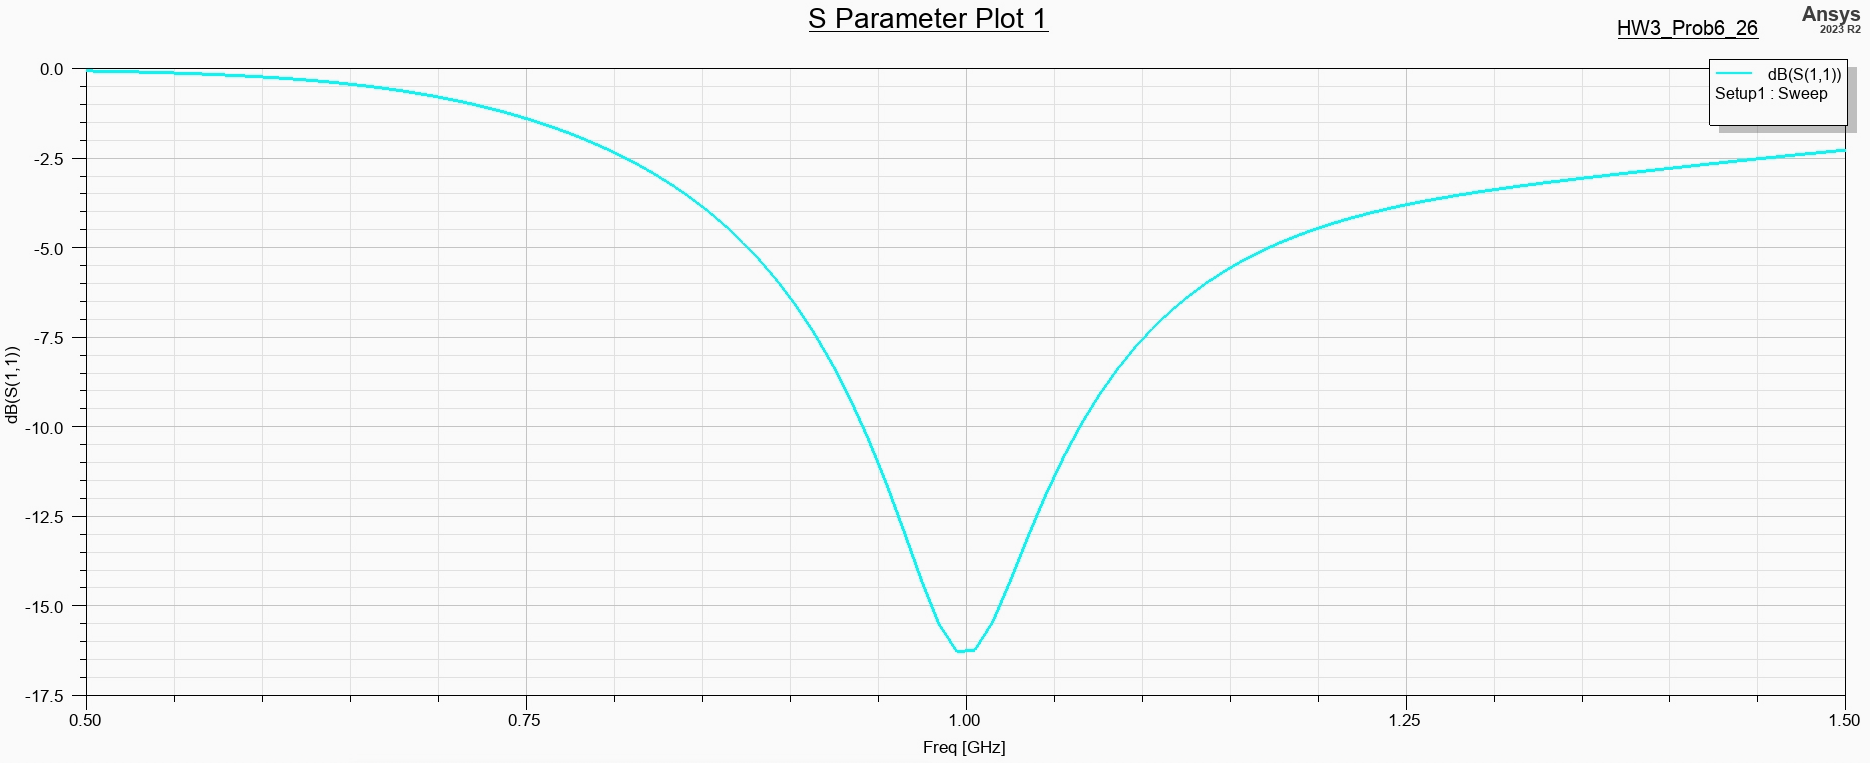
\includegraphics[width=15cm]{./images/6-26.png}
    \caption{S11 results of antenna}
    \label{fig:S11}
  \end{figure}
\end{center}
\begin{center}
\begin{figure}[h]
    \centering
    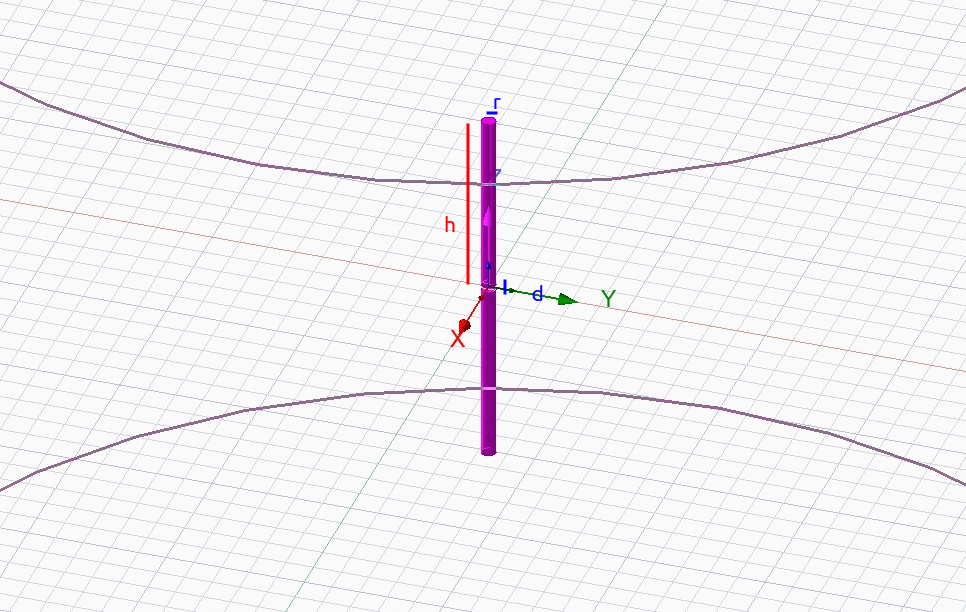
\includegraphics[width=15cm]{./images/model.png}
    \caption{model of antenna}
    \label{fig:Model}
  \end{figure}
\end{center}
\begin{center}
Final dimensions found by optimization to get the best match:\\$l= 2 \cdot h =132.24$mm\\$r=2.606$mm\\$d=2.09$mm
\end{center}
I am not entirely sure how I would verify this in HFSS, but I did put together the antenna and here are the results/model. 
\newpage
\section{- 6.38}
A coaxial line of inner and outer radii $a$ and $b$, respectively, is mounted on an infinite
conducting ground plane. Assuming that the electric field over the aperture of the coax is:
\[
E_a = -\hat{a}_{\rho} \frac{V}{\varepsilon \ln(\frac{b}{a}) \rho\ '}
\]
\begin{center}
  $\text{where } a \leq \rho\ ' \leq b$
\end{center}
where V is the applied voltage and $\epsilon$ is the permittivity of medium in the coax, find the far-zone spherical electric and magnetic field components radiated by the aperture.
\begin{center}
  \begin{tikzpicture}[scale=2,tdplot_main_coords]

    % Define the radii
    \def\innerradius{0.5}
    \def\outerradius{1}
    \def\ellipseangle{0}

    % Draw the annulus as ellipses due to the perspective
    \begin{scope}[rotate=\ellipseangle]
        \shade[inner color=gray!80,outer color=gray!30,opacity=0.75] (0,0) ellipse ({\outerradius} and {0.5*\outerradius});
        \fill[white] (0,0) ellipse ({\innerradius} and {0.3*\innerradius});
    \end{scope}

    % Draw the outer shaded area
    \fill[gray!30,opacity=0.5] (-1.5,-1.5) rectangle (1.75,1.75);

    % Draw the arrows and labels
    \draw[-{Latex[length=3mm]}] (0,0) -- (2.5,0) node[anchor=south east] {$y$};
    \draw[-{Latex[length=3mm]}] (0,0) -- (0,2.5) node[anchor=north west] {$z$};
    \draw[-{Latex[length=3mm]}] (0,0) -- (-1.5,-1.5) node[anchor=north] {$x$};

    % Label the radii and other parameters
    \begin{scope}[rotate=\ellipseangle]
        \draw (0,0) -> node[midway,above] {$a$} (-\innerradius/2,.15);
        \draw (0,0) -> node[midway,above] {$b$} ({-\outerradius/2},.45);
    \end{scope}
    \node[anchor=south] at (0,-.5) {$\varepsilon$};
    \node at (1.3,-1.3) {$\sigma = \infty$};

    % Label the figure
    \node[below] at (current bounding box.south) {Figure P6-38};
\end{tikzpicture}
\end{center}
\newpage
\textcolor{white}{  }
\newpage
\newpage
\textcolor{white}{  }
\newpage

\section{- 7.3}
An infinitesimal vertical magnetic dipole of length l and constant current Im is placed symmetrically about the origin and it is directed along the z axis, as shown in Figure 6-2 a. Derive expressions valid every- where, near and far field, for the:
\begin{itemize}
\item Electric vector potential components $(F_r , F_{theta} , F_{phi} )$.
\item Electric field components $(E_r , E_{theta} , E_{phi} )$.
\item Magnetic field components $(H_r , H_{theta} , H_{phi} )$.
\item Time-average power density, defined as \\
  \begin{align*}
  \mathbf{S} = \frac{1}{2}\text{Re}{[\mathbf{E}\times\mathbf{H}^*]}
  \end{align*}
\item  Radiation intensity, defined in the far field $U \approx r^2S_{av}$
  \item Power Radiated, defined as \\
  \begin{align*}
  \mathbf{P}_{rad} = \int_0^{2\pi}\int_0^{\pi}U(\theta,\phi)\sin{(\theta)}d\theta d\phi
  \end{align*}
\item Maximum directivity, defined as:
  \begin{align*}
  \mathbf{D}_{0} = \frac{4\pi U(\theta,\phi)}{\mathbf{P}_{rad}}
  \end{align*}
\item Radiation resistance, defined as:
  \begin{align*}
  \mathbf{R}_{r} = \frac{2\mathbf{P}_{rad}}{|I_m|^2}
  \end{align*}
\end{itemize}
\newpage
\textcolor{white}{  }
\newpage
\textcolor{white}{  }
\newpage

\section{- 7.15}
An infinitesimal electric dipole is placed at an angle of $30\degree$ at a height $h$ above a perfectly conducting electric ground plane. Determine the location and orientation of its image. Do this by sketching the image.
\begin{center}
  \begin{tikzpicture}

    % Ground
    \fill[gray!50] (-2,-2) rectangle (2,0);
    \draw (-2,0) -- (2,0);

    % Sigma = infinity
    \node at (1,-0.5) {$\sigma = \infty$};

    % Antenna
    \draw[thick, dotted] (0,1.25) -- (1.5,1.25);
    \draw[->,thick] (0,1) -- +(30:1) node[midway, above right, xshift=.5em, yshift=.5em] {30$^\circ$};
    \fill (.425,1.25) circle (1pt);
    % Height
    \draw[<->] (-0.5,0) -- node[midway, fill=white] {$h$} (-0.5,1.25);

    % Label
    \node[below] at (0,-2.5) {Figure P7-15};
\end{tikzpicture}
\end{center}
\begin{center}
  \begin{tikzpicture}

    % Ground
    \fill[green!20] (-2,-2) rectangle (2,0);
    \draw (-2,0) -- (2,0);

    % Sigma = infinity
    \node at (1,-1.9) {$\sigma = \infty$};

    % Antenna
    \draw[thick, dotted] (0,-1.15) -- (1.5,-1.15);
    \draw[->,thick] (.8,-1.4) -- +(150:1) node[midway, above right, xshift=.5em, yshift=.5em] {};
    \fill (.425,-1.15) circle (1pt);
    % Label
    \node[below] at (0,-3) {Solution};
\end{tikzpicture}
\end{center}
\newpage
\section{- 7.37}
For the aperture shown in Figure 6-4c and assuming it is mounted on an infinite PEC ground plane:
\begin{itemize}
\item [a)] Form the most practical, exact or approximate (when necessary to solve the problem), equivalent currents $\mathbf{J}_s$ and $\mathbf{M}_s$.
\item [b)] Find the far-zone electric and magnetic fields. The electric field distribution at the aperture is given by ($Eo$ is a constant):\\
  \begin{align*}
    \mathbf{E}_a &= \hat a_yE_0\\
    -\frac{a}{2} \le x\ ' \le \frac{a}{2}\ \ \ &;\ \ \ -\frac{b}{2} \le y\ ' \le \frac{b}{2}
  \end{align*}
\end{itemize}
\newpage
\textcolor{white}{  }
\newpage

\bibliographystyle{plain}
\bibliography{references/references}

\end{document}

%%% Local Variables:
%%% mode: LaTeX
%%% TeX-master: t
%%% End:
